\chapter{Complex Attosecond Transient-absorption Spectroscopy}
\label{chap:CATS}

\section{Introduction}
\label{sec:intro_cats}

As seen in Chapter \ref{chap:ATS}, a rich amount of information can be extracted from ATS experiments.  Specifically, dynamics such as light-induced states and strong-field ionization of  excited states induced by a dressing field can be deduced from the change in photoabsorption cross section.  However, these experiments are limited by the fact that they only have access to the imaginary part of the complex refractive index of the medium of interest. There should also be a corresponding change in the real part of the complex refractive index that remains unobserved.  In this Chapter, the techniques introduced in Chapters \ref{chap:two_source} and \ref{chap:refractive_index} are extended to measure both parts of the complex refractive index in the experiments performed in Chapter \ref{chap:ATS}.  This new method to measure the change in the complex refractive index induced by a dressing field will be referred to as Complex Attosecond Transient-absorption Spectroscopy (CATS).


\section{Theory}
\label{sec:cats_theory}

In ATS experiments, such as those described in Chapter \ref{chap:ATS}, the dynamics induced by a dressing field is imprinted upon the photoabsorption cross section and, macroscopically, the optical density (OD) of the sample \cite{wuTheoryStrongfieldAttosecond2016,geneauxromainTransientAbsorptionSpectroscopy2019}.  Measuring a change in the OD of the sample yields a rich amount of information, however it does not represent a direct measurement of all the of the changes induced in the sample. 


\begin{equation}
	\label{eqn:MWE}
	\nabla_{\perp}^{2}\tilde{\mathcal{E}}(\omega) + \frac{2i\omega}{c}\frac{\partial \tilde{\mathcal{E}}(\omega)}{\partial z} = -\frac{\omega^2}{\epsilon_0 c^2}\tilde{P}(\omega)
\end{equation}


\begin{equation}
	\label{eqn:MWE_polarization_def}
	\tilde{P}(\omega) = 2\rho\tilde{d}(\omega) = 2\rho\tilde{\mathcal{E}}(\omega)\Bigg(\mathrm{Re}\bigg[\frac{\tilde{d}(\omega)}{\tilde{\mathcal{E}}(\omega)}\bigg] + i \mathrm{Im}\bigg[\frac{\tilde{d}(\omega)}{\tilde{\mathcal{E}}(\omega)}\bigg]\Bigg)
\end{equation}

\begin{equation}
	\label{eqn:MWE_linear_resp}
	\frac{2i\omega}{c}\frac{\partial \tilde{\mathcal{E}}(\omega)}{\partial z} = -\frac{\omega^2}{\epsilon_0 c^2}\tilde{P}(\omega)
\end{equation}


Specifically, the $\dod$ only captures the change in the imaginary part of the dipole, as can be seen by the relationship
\begin{equation}
	\label{eqn:dod_im_dipole}
	\dod(\omega) = \frac{\rho L}{\ln 10}\big(\sigma_{\mathrm{on}}(\omega) - \sigma_{\mathrm{off}}(\omega)\big) = \frac{8\pi\rho l \omega}{\ln 10}\Bigg( \mathrm{Im}\Bigg[\frac{\tilde{d}_{\mathrm{on}}(\omega)}{\tilde{\mathcal{E}}(\omega)}\Bigg] - \mathrm{Im}\Bigg[\frac{\tilde{d}_{\mathrm{off}}(\omega)}{\tilde{\mathcal{E}}(\omega)}\Bigg] \Bigg),
\end{equation}
where $\rho$ is the density of the sample, $L$ is the medium length, $\tilde{d}(\omega)$ is the dipole moment in the frequency domain, and $\tilde{\mathcal{E}}(\omega)$ is the combined electric field of the XUV APT and the IR dressing pulse. Therefore measuring the $\dod$ only leads to a direct measurement of half of the total information possible because the real part of the dipole is unknown.  The change in the real part of the dipole is macroscopically related to a change in the real part of the complex refractive index, and this relationship is given by 
\begin{equation}
	\label{eqn:dn_re_dipole}
	\Delta n(\omega) = 4\pi \rho \Bigg( \mathrm{Re}\Bigg[\frac{\tilde{d}_{\mathrm{on}}(\omega)}{\tilde{\mathcal{E}}(\omega)}\Bigg] - \mathrm{Re}\Bigg[\frac{\tilde{d}_{\mathrm{off}}(\omega)}{\tilde{\mathcal{E}}(\omega)}\Bigg] \Bigg).
\end{equation}


!!!!!!! Add section here with the derivation of the change in real and imaginary parts from Gaarde/Wu!!!!!!!!!!

\begin{equation}
	\label{eqn:complex_refractive_index)}
	\tilde{n} = \big(n+\Delta n\big) + i \big(\beta + \Delta\beta\big)
\end{equation}

\subsection{Direct Measurement}

To directly measure this expected change in the real part of the refractive index there are a few methods that can be applied.  One technique that is often used is an interferometric method to measure the change in refractive index as a phase shift between two arms of a Mach-Zehnder interferometer, and this concept was introduced in detail in Chapter \ref{chap:refractive_index}. In general, interferometric techniques are technically challenging in this wavelength range because of a lack of broadband and efficient optics and a high interferometric stability required by the relatively short wavelengths.  There are a few methods to overcome these challenges, and they generally can be divided into two different approaches: either splitting the XUV beam after it is generated (for example, with split mirrors \cite{nabekawaInterferometricAutocorrelationAttosecond2008, nabekawaInterferometryAttosecondPulse2013}) or generating two nearly identical XUV beams that can be interferred (for example, with a Michelson interferometer before generation of the XUV \cite{kovacevExtremeUltravioletFourierTransform2005}).  In Chapter \ref{chap:two_source}, it was shown how the later approach can be implemented using a SWPG that is able to control the relative phase of the two generated XUV beams.  Furthermore, in Chapter \ref{chap:refractive_index} it was demonstrated that this setup can be used to measure the refractive index of two different materials by measuring a phase shift between the two generated XUV sources over a broad energy range.  In that case, the phase shift induced by the sample was known \textit{a priori} because the ground state refractive index has been well characterized previously, and the excellent agreement between the extracted refractive index and the known refractive index demonstrated the validity of this technique.  

\begin{figure}
	\centering
	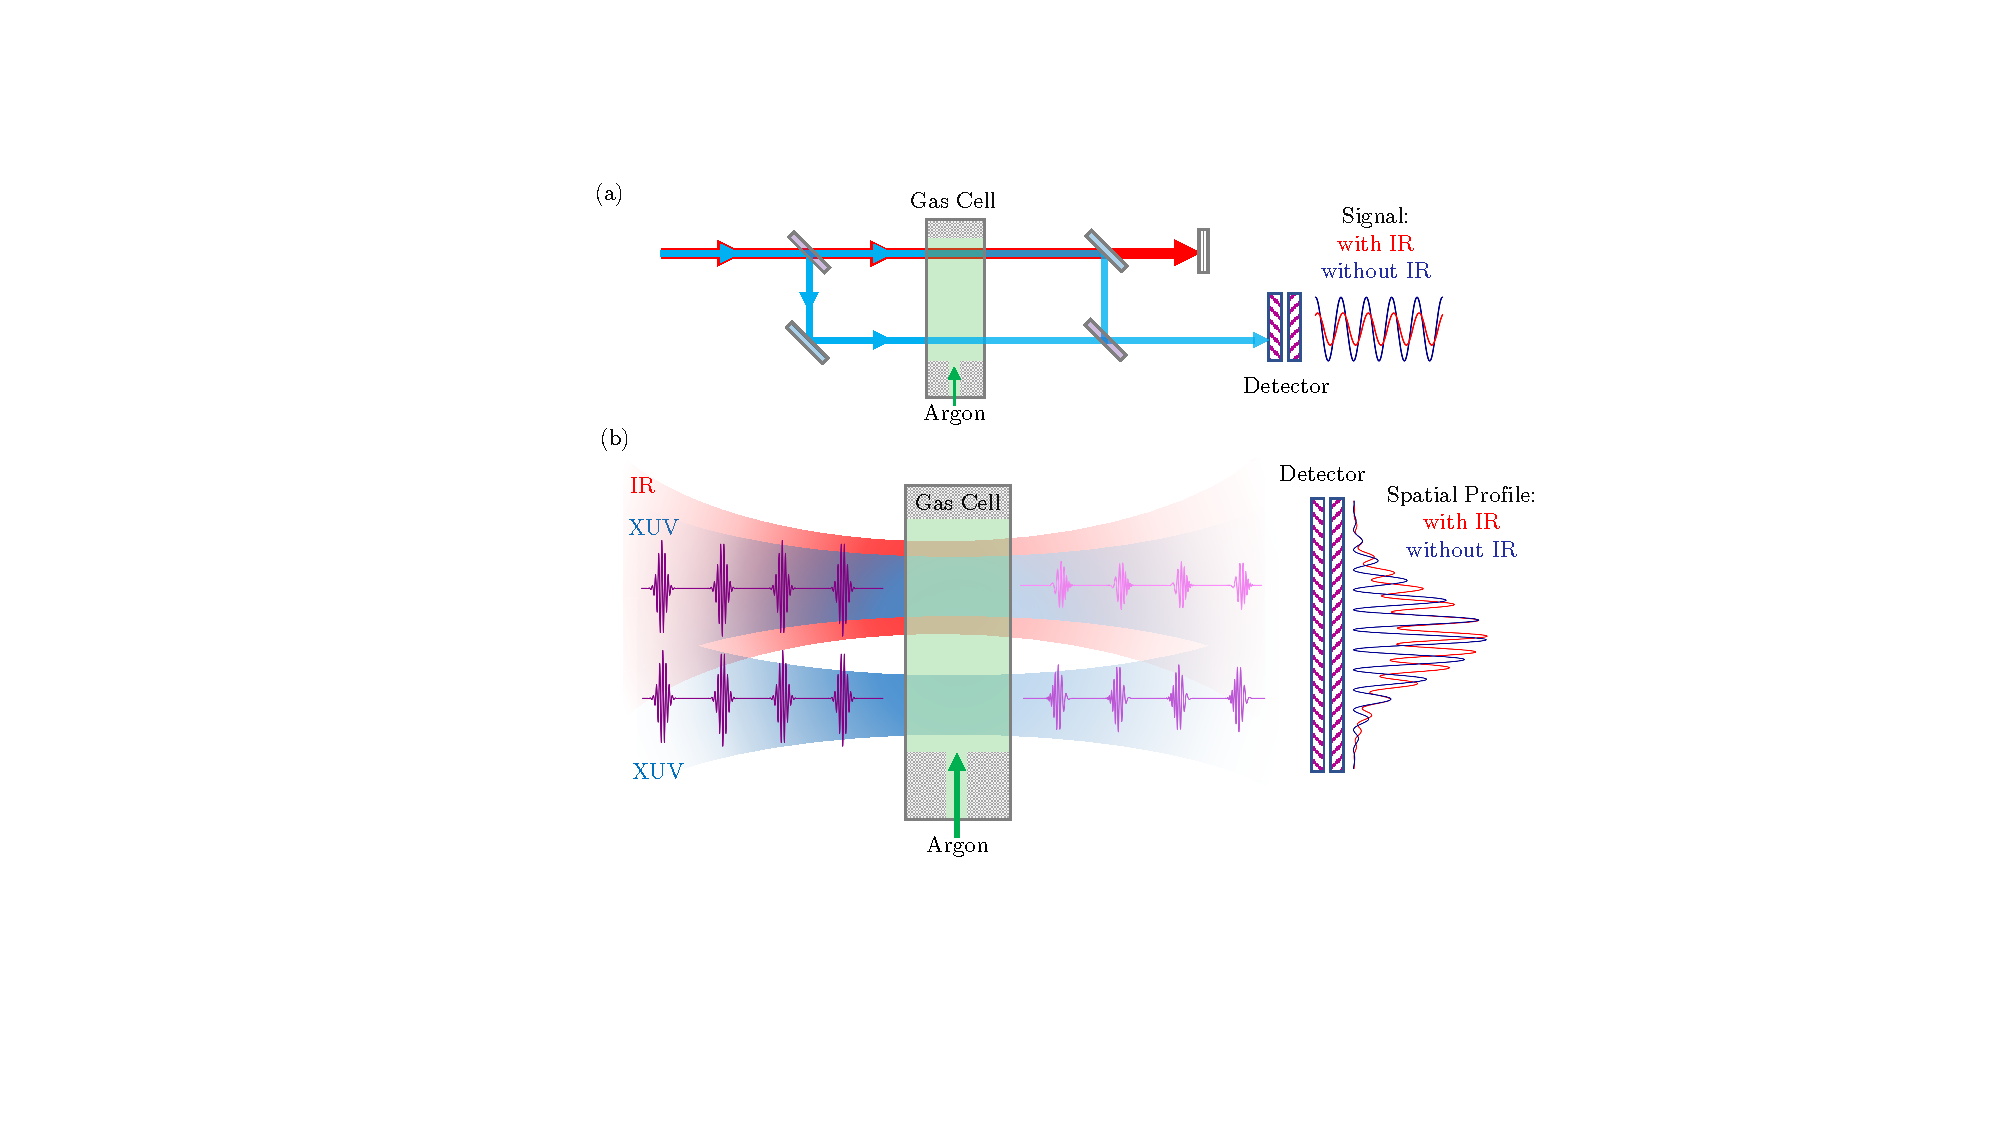
\includegraphics[width=1.0\textwidth]{figures/CATS/CATS_mach_zehnder.pdf}
	\caption[Schematic of Mach-Zehnder interferometer and spatial profile with and without an IR dressing field in one arm of the interferometer]{(a) Schematic of a Mach-Zehnder interferometer that is used to measure the phase shift induced by an IR dressing field introduced into one of the arms of the interferometer. (b) For the experiments described in this chapter, the two XUV sources generated by a SWPG will act as the two arms of a Mach-Zehnder interferometer, and the sample of interest will only be dressed in one the sources by an IR field.}
	\label{fig:CATS_mach-zehnder_interferometer}
\end{figure}

In the experiment presented in Chapter \ref{chap:refractive_index}, the complex refractive index that was measured corresponded to the ground state of a material.  However, this method can be generalized to measure more than just the static ground state, and it can be used to measure a dynamically induced change in refractive index via a dressing pulse.  The basic principle is shown schematically in figure \ref{fig:CATS_mach-zehnder_interferometer}, and it involves inducing a phase shift in only one arm of a Mach-Zehnder interferometer that is comprised of two nearly identical XUV beams going through the same medium. In a manner that is the same as what was presented in Chapter \ref{chap:refractive_index}, these two XUV beams will be generated by a SWPG.  The inherent interferometric stability of the SWPG due to its single-optic operation allows for measurements of phase shifts between the two beams that correspond to a delay of only a few attoseconds (see figure \ref{fig:interferogram_ge} for an example) that arise due to the change in the real refractive index induced by the dressing pulse.  The relationship between the change in the real refractive index, $\Delta n$, and the phase shift between the two beams, $\Delta\phi$, is given by
\begin{equation}
	\label{eqn:phase_shift_dn}
	\Delta \phi = \frac{2\pi L \Delta n}{\lambda}
\end{equation}
for a medium of length $L$.  This phase shift between the two beams is directly measured as a fringe shift in the spatial profile of interference pattern in the far-field, as was shown previously. This combined with a spectrometer allows for the measurement of the induced phase shift as a function of photon energy, and consequently, the real part of the refractive index can be measured as a function of photon energy.  

Additionally, the change in the imaginary part of the refractive index induced by the dressing pulse will lead to a change in absorption between the two beams, and this will lead to a change in fringe contrast in the far-field interference pattern.  The relationship between the change in contrast and the change in the imaginary refractive index, $\Delta \beta$,  is given by
\begin{equation}
	\label{eqn:beta_fringe_contrast_chap_cats}
	\Delta\beta = -\frac{\lambda}{2\pi L} \ln\Bigg[\frac{V_0}{V}\Bigg(1-\sqrt{1-\bigg(\frac{V}{V_0}\bigg)^2}\Bigg)\Bigg]
\end{equation}
where $V_0$ is the fringe contrast without the dressing pulse present and $V$ is the contrast with the dressing pulse present.  This change in imaginary part of the refractive index is related to the change in absorption, $\dod$, by the relationship
\begin{equation}
	\label{eqn:dod_to_beta}
	\dod(\lambda) = \frac{4\pi L}{\lambda \ln 10}\Delta \beta(\lambda),
\end{equation}
when the Beer-Lambert Law is assumed to hold true. 

Therefore, just as in the experiment performed in Chapter \ref{chap:refractive_index}, it is possible to directly measure the complex refractive index using a SWPG to generate an inline interferometer between two nearly identical XUV beams.  The primary difference is that now we are measuring only a change in the complex refractive index induced by a dressing pulse, as opposed to the total complex refractive index which would include the ground state.  This is due to the fact that this measurement is inherently differential in nature.  To measure the total complex refractive index, then one would have to limit the medium that is being dressed to only one of the two sources.  This is technically challenging for a gas sample, so only the change in complex refractive index is measured in this chapter.


\subsection{Indirect calculation: Kramers-Kronig Relations}

\section{Complex Attosecond Transient-absorption Spectroscopy of Fano resonances}
\label{sec:CATS_ar}

\subsection{Experimental setup}
\label{sec:CATS_ar_exp_setup}

\begin{figure}
	\centering
	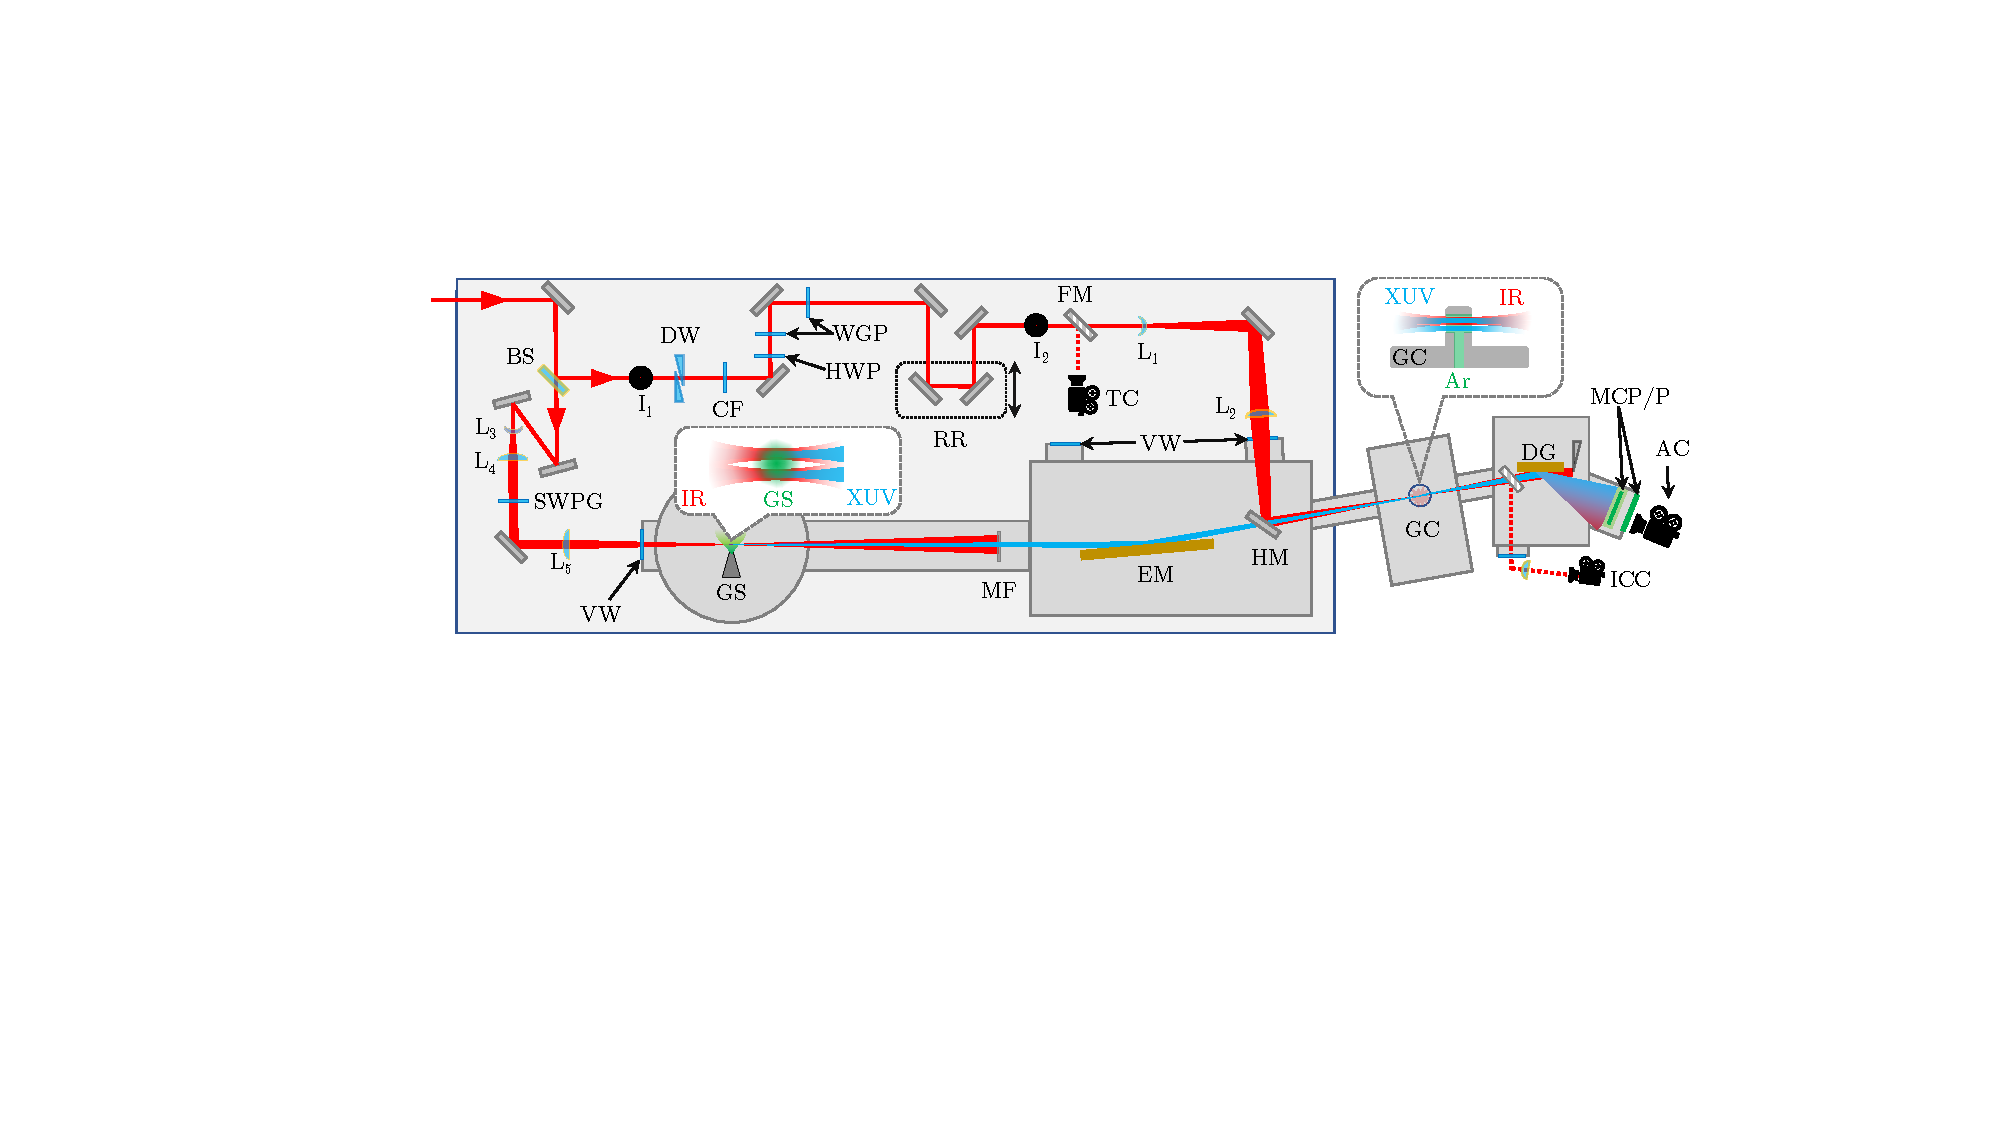
\includegraphics[width=1.0\textwidth]{figures/CATS/beamline_schematic_CATS.pdf}
	\caption[TABLe experimental setup for ATS experiments]{Schematic of the optical setup for the experiments described in this chapter.  \textbf{BS}: Beamsplitter (Thorlabs BSF20-C), \textbf{I$_{1,2}$}: Irises used for alignment. \textbf{DW}: Delay wedges for fine delay control. \textbf{CF}: Color filter (Thorlabs FELH1000). \textbf{HWP}: Half-wave plate. \textbf{WGP}: Wire grid polarizer. \textbf{RR}: Retro reflector for coarse delay adjustment.  \textbf{FM}: Flip mirror. \textbf{TC}: Thermal camera used for alignment.  \textbf{L$_1$}: $f=-300$ mm lens (Thorlabs LF1015-C). \textbf{L$_2$}: $f=500$ mm lens (Thorlabs LA1380-C). \textbf{VW}: Vacuum window, 3 mm CaF$_2$, \textbf{HM}: Hole mirror with 10 mm hole.  \textbf{L$_3$}: $f=-400$ mm lens.  \textbf{L$_4$}: $f=500$ mm lens. \textbf{L$_5$}: $f=400$ mm lens.  \textbf{BBO}: Second-harmonic generation crystal.  \textbf{Cal}: Calcite. \textbf{GS}: Gas source for HHG. \textbf{MF}: Aluminum filter. \textbf{EM}: Ellipsoidal mirror. \textbf{GC}: Gas cell. \textbf{RM}: Removable mirror for \textit{in-situ} diagnotics.    \textbf{ICC}: camera for \textit{in-situ} diagnotics. \textbf{DG}: VLS diffraction grating. \textbf{BB}: Baffles to block zero order diffraction.  \textbf{MCP/P}: Microchannel plate and phosphor.  \textbf{AC}: Andor Neo 5.5 CMOS camera.}
	\label{fig:CATS_setup}
\end{figure}



\subsection{Results}
\label{sec:CATS_ar_results}


\section{Conclusion}
\label{sec:CATS_conclusion}